\chapter{Introdu\c{c}\~ao e teoria}

%\section{Motiva\c{c}\~ao}

% DIZER ALGO SOBRE COMO SERA O SISTEMA, COM BARRAS E CONEXOES E QUE FICA COMPLEXO SEM ANALISE DE FLUXO DE CARGA Mas como \'e possivel garantir o planejamento e opera\c{c}\~ao sistema de grandes propor\c{c}\~oes como esse? Para isso, \'e preciso saber o estado atual do sistema. Por\'em, n\~ao \'e vi\'avel medir todos os pontos de interesse. Isso seria custoso e tomaria muito tempo. 


%Para  como um todo \'e necessario que tenhamos ferramentas que nos ajudem a estimar o estado da rede 

%\section{Introdução à Teoria}
A ferramenta de an\'alise de sistemas de energia el\'etrica aqui discutida ser\'a a An\'alise de Fluxo de Pot\^encia. Essa an\'alise nos fornecer\'a um metodo de cálculo de importantes grandezas de todo o sistema, a partir de algumas grandezas conhecidas, ou seja, que podem ser medidas. Esta \'e uma ferramenta aplicada \`a um sistema est\'atico.  \cite{monticelli}
\section{Modelagem}
\label{SectionIntro}
Toda a rede ser\'a composta por ramos e barras, onde ramos s\~ao a representa\c{c}\~oes das linhas de transmiss\~ao e transformadores. As barras s\~ao n\'os do sistema e nesses pontos de interesse, pode-se medir fisicamente algumas grandezas, a depender do tipo de barra. S\~ao definidas quatro vari\'aveis \`a para cada k-ésima barra, correspondentes \`a tens\~ao e \`a inje\c{c}\~ao de
pot\^encia nesta barra, $V_k$, magnitude da tens\~ao nodal, $\theta_k$ angulo da tens\~ao nodal, $P_k$ inje\c{c}\~ao l\'iquida de pot\^encia ativa e $Q_k$ inje\c{c}\~ao l\'iquida de pot\^encia reativa. As barras s\~ao divididas em categorias como na tabela \ref{t_PQPVSlack} de acordo com as grandezas conhecidas e suas incognitas.
\begin{table}[]
\caption{Categoria das barras de acordo com variáveis conhecidas}
\begin{tabular}{@{}llll@{}}
\toprule
Tipo & Dados & Incógnitas & Caracteristicas \\ 
\midrule
$PQ$ & $P_k$,$Q_k$ & $V_k$,$\theta_k$  & Barra de carga \\
$PV$ & $P_k$,$V_k$ & $Q_k$,$\theta_k$  & Barra de geração\\
Referência (Slack) & $V_k$,$\theta_k$ & $P_k$,$Q_k$& Barra de geração em grandes fornecedoras \\ \bottomrule
\end{tabular}
\label{t_PQPVSlack}
\end{table}



\section{Formula\c{c}\~ao do problema b\'asico}
\label{SectionFormula}
\subsection{Injeção de potências}

Seja uma rede de energia gen\'erica que cont\'em um n\'umero de barras \textit{(NB)} arbitr\'ario. Para cada barra, \'e poss\'ivel escrever duas equa\c{c}\~oes de inje\c{c}\~oes de pot\^encia, como em \ref{Pk} e \ref{Qk}. Elas são obtidas ao aplicar Lei de Kirchhoff das correntes em todas as $NB$ barras do sistema.\\
\begin{equation}
    P_k = V_k \sum_{m\in \kappa} V_m (G_{km} cos\theta_{km} + B_{km}sen\theta_{km})
    \label{Pk}
\end{equation}
\begin{equation}
    Q_k = V_k \sum_{m\in \kappa} V_m (G_{km} sen\theta_{km} - B_{km}cos\theta_{km})
    \label{Qk}
\end{equation}
Portanto, em um sistema com \textit{NB} barras, \'e possivel obter $2.NB$ equa\c{c}\~oes.\\
Neste problema, utilizaremos como variáveis de estado, ou seja, nosso conjunto de incognitas que descreverão o sistema, as variáveis $V$ e $\theta$, representados em \ref{Vs} e \ref{TetaS}. Com esses valores resolvidos, \'e possível calcular todas as injeções de potência em todas as barras.\\
\begin{equation}
    V^S  = \left[ \begin{matrix} V_1^S & V_2^S & V_3^S & ... & V_{NB}^S  \end{matrix} \right]^T 
    \label{Vs}
\end{equation}

\begin{equation}
    \theta^S  = \left[ \begin{matrix} \theta_1^S & \theta_2^S & \theta_3^S &... & \theta_1^S  \end{matrix} \right]^T 
    \label{TetaS}
\end{equation}
Quando \ref{Vs} e \ref{TetaS} forem resolvidas, será possivel aplicar em \ref{Pk} e \ref{Qk} para se obter \ref{Pk_s} e \ref{Qk_s}, que será as injeções de potência para o estado atual da rede.
\begin{equation}
    P_k = V_k^S \sum_{m\in \kappa} V_m^S (G_{km} cos\theta_{km}^S + B_{km}sen\theta_{km}^S)
    \label{Pk_s}
\end{equation}
\begin{equation}
    Q_k = V_k^S \sum_{m\in \kappa} V_m^S (G_{km} sen\theta_{km}^S - B_{km}cos\theta_{km}^S)
    \label{Qk_s}
\end{equation}
Problema consiste em obter o estado $(V^S,\theta^S)$.\\
Com um simples algebrismo matemático, as equações \ref{Pk} e \ref{Qk} serão representas aqui como em \ref{Pk_balanceado} e \ref{Qk_balanceado}.
\begin{equation}
    P_k - V_k \sum_{m\in \kappa} V_m (G_{km} cos\theta_{km} + B_{km}sen\theta_{km}) = 0
    \label{Pk_balanceado}
\end{equation}
\begin{equation}
    Q_k - V_k \sum_{m\in \kappa} V_m (G_{km} sen\theta_{km} - B_{km}cos\theta_{km}) = 0
    \label{Qk_balanceado}
\end{equation}

%essas equaoces tem que dar 0 pois são dua coisas iguais

%dada uma rede qualquer, o nume de equacoes sera XXXX colocar 

%inserir tahbelas tipos de barras

%numero de equacoes = numero de incognitas e o sistema é LI. POrtante há solução

%do ponto de vista didático

\subsection{Matriz de Admitância}
Seja a matriz de admitância nodal $Y$ e ela se relacione com o vetor de tensões nodais $V$ e vetor de injeções de corrente nodais $I$ da forma como em \ref{Admitancia}.
\begin{equation}
    I = Y.V
    \label{Admitancia}
\end{equation}
A regra de formação dessa matriz $Y$ será dada por \ref{AdmitanciaElementosForaDiagonal} e \ref{AdmitanciaElementosDiagonal} (A dedução desse conjunto de formulas não será abordado neste trabalho).\\
A dimensão da matriz $Y$ será de $NB$x$NB$.\\
Para os elementos fora da diagonal principal, será o valor negativo da admitância série entre as duas barras, como em \ref{AdmitanciaElementosForaDiagonal}.
\begin{equation}
    Y_{km} = -y_{km}
    \label{AdmitanciaElementosForaDiagonal}
\end{equation}
Para os elementos na diagonal principal, será a soma das admitâncias conectadas à barra, como em \ref{AdmitanciaElementosDiagonal}, onde $\Omega_k$ é o conjunto de barras vizinhas da barra $k$.
\begin{equation}
    Y_{kk} = \sum_{m\in \Omega_k} \left(y_{km} + j\frac{b^{sh}_{km}}{2}\right)
    \label{AdmitanciaElementosDiagonal}
\end{equation}
Ainda, a matriz $Y$ será dividida em parte real(\ref{G}) e parte imaginária (\ref{B}). Dando origem às matrizes de condutância $G$ e susceptância $B$, usadas nas equações de injeção de potência \ref{Pk} e \ref{Qk}.
\begin{equation}
    G = \mathbb{R} (Y)
    \label{G}
\end{equation}
\begin{equation}
    B = \mathbb{I} (Y)
    \label{B}
\end{equation}

\section{Método linearizado}
\label{SecaoMetodoLinearizado}
O método de Fluxo de potência linearizado ou CC, é um método que permite calcular, com baixo custo computacional, e precisão aceitável para algumas aplicações, a distribuição dos fluxo de potência ativa em redes de transmissão (extra-alta tensão e ultra-alta-tensão). Neste método, que se baseia na alta correlação entre entre a Potência Ativa e o ângulo da tensão \cite{raphael}.\\
Importante: este é um método para potência ativa, ou seja, esse método não será usado para potência reativa.\\
No trabalho anterior, foi utilizado uma simplificação para o fluxo de potência ativa. O fluxo de potência ativa pode ser como em \ref{Pkm_linearizado}.\\
Antes, como hipóteses para simplificação, utiliza-se apenas a potência ativa e desconsidera-se as perdas ativas e tem-se \ref{Pk_linearizadoSimplificado1}.
\begin{equation}
    P_{km} = G_{km}V^2_{k}-V_k.V_m (G_{km} cos\theta_{km} + B_{km}sen\theta_{km})
    \label{Pk_linearizadoSimplificado1}
\end{equation}
Considerando, então, as tensões iguais a $1pu$, tem-se \ref{Pk_linearizadoSimplificado2}.
\begin{equation}
    P_{km} = -B_{km}sen\theta_{km}
    \label{Pk_linearizadoSimplificado2}
\end{equation}
Por fim, linearizando a senoide com $sen\theta_{km} \approx \theta_{km} \approx (\theta_{k} - \theta_{m})$, tem-se \ref{Pkm_linearizado}.
\begin{equation}
    P_{km} \approx  k_1.\theta_{km} \approx \frac{1}{x_{km}}.(\theta_k - \theta_m)
    \label{Pkm_linearizado}
\end{equation}
Ou seja, é aproximadamente proporcional à abertura angular da linha e desloca-se no sentido dos ângulos maiores para menores ($P_{km}>0$ se $\theta_k > \theta_m$) \cite{castro}.\\
A partir de \ref{Pkm_linearizado}, pode-se calcular a injeção liquida de potência em cada barra como em \ref{Pk_linearizado_InjecaoLiquida}.
\begin{equation}
    P_{k} = \sum_{m\in\Omega_k} P_{km}
    \label{Pk_linearizado_InjecaoLiquida}
\end{equation}
Em termos matriciais, \ref{Pkm_linearizado} pode ser reescrito como em \ref{Pk_linearizado_InjecaoLiquida_Matricial}
\begin{equation}
    \left[ \begin{matrix} P \end{matrix} \right] =  \left[ \begin{matrix} B' \end{matrix} \right] .  \left[ \begin{matrix} \theta \end{matrix} \right]
    \label{Pk_linearizado_InjecaoLiquida_Matricial}
\end{equation}
A matriz $B'$ será escrita seguindo a regra de formação dada em \ref{Blinhalinearizado_km} e \ref{Blinhalinearizado_kk}
\begin{equation}
    B'_{km} = -\frac{1}{x_{km}}
    \label{Blinhalinearizado_km}
\end{equation}
\begin{equation}
    B'_{kk} = \sum_{m\in \Omega_k} \left(\frac{1}{x_{km}}\right)
    \label{Blinhalinearizado_kk}
\end{equation}

%%%%%%%%%%%%%%%%%%%
\section{Algoritmo implementado}

Aqui será utilizado um algoritmo discutido nos slides do Professor Castro. \cite{castro}.
\subsection{Método linearizado}
\label{SubsectionMetodoLinearizado}
\begin{enumerate}
    \item Calcula-se agora a equação \ref{Pk_linearizado_InjecaoLiquida_Matricial}.
    \item Calcula-se a matriz P, com os valores dados.
    \item Calcula-se a matriz $B'$, como descrito em \ref{Blinhalinearizado_km} e \ref{Blinhalinearizado_kk}. Pode-se, também, obter a matriz B' atravez da parte imaginária da matriz de admintânica Y (\ref{B}). Neste caso, é necessário desconsiderar a linha e a coluna da barra de referência (slack). 
    \item Calcula-se a transposta de $B'$. 
    \item Multiplica-se $[B']^T.[P]=[\theta]$
    \item Calcula-se os fluxos de potência. O fluxo de potência da barra $k$ e a barra $m$ será dado por $P_{km} = (\theta_k - \theta_m)/x_{km}$ como na figura \ref{FigFluxoPotenciaLinearizado}
        \begin{figure}[!htb]
            \caption{Fluxo de potência aproximado. \cite{castro}}
            \centering % para centralizarmos a figura
            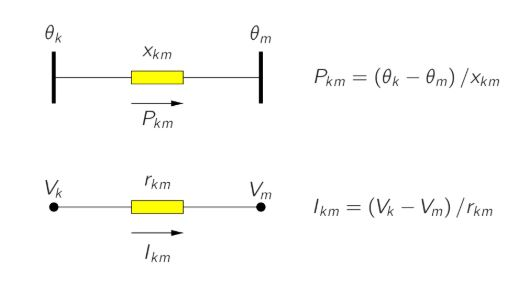
\includegraphics[width=8cm]{figuras/FluxoLinearizado.JPG}
            \label{FigFluxoPotenciaLinearizado}
        \end{figure}
    \item Converte-se os angulos para graus, dado que estão em radianos.
\end{enumerate}
